\documentclass{article}
\usepackage[UTF8]{ctex}
\usepackage{geometry}
\usepackage{listings}
\usepackage{fancyhdr}
%\usepackage[colorlinks,linkcolor=blue]{hyperref} 

%\usepackage{amsmath}
\usepackage{graphicx}
%\usepackage{pgfplots}

\geometry{left = 2cm,right = 2cm,top = 3cm,bottom = 3cm}
\pagestyle{fancy}
\fancyhf{}
\fancyhead[R]{\leftmark}
\fancyhead[L]{\rightmark}
\fancyhead[C]{多周期处理器}
\fancyfoot[C]{\thepage}
\renewcommand{\headrulewidth}{0.2mm}

\title{数字逻辑与处理器基础\\多周期处理器}

\author{cvxbzn}

\begin{document}

\maketitle

\section{数字通路设计}
\subsection{寄存器与多路选择器及其功能}
\begin{itemize}
    \item 寄存器
          \begin{itemize}
              \item PC:输入下一状态PC,输出当前PC,使能信号为1时在时钟上升沿写入。
              \item 指令寄存器(IR):存放从存储器中取出的指令,IRWrite为1时在时钟上升沿写入
              \item 数据寄存器(MDR):输入存储器的输出MemData。
              \item 临时寄存器A:输入为寄存器堆中的ReadData1
              \item 临时寄存器B:输入为寄存器堆中的ReadData2
              \item ALU寄存器ALUOut:存放ALU输出ALUOut
          \end{itemize}
    \item 多路选择器
          \begin{itemize}
              \item IorD:Instruction or data,选择读取存储器的数据为指令(0)或者数据(1)。
              \item RegDst:选择写回寄存器堆中的寄存器位置,rt(00),rd(01)或者\$ra(10),其中\$ra在执行jal指令时使用。
              \item MemToReg:选择写回寄存器堆的数据来源。ALUOut(00),内存数据(01),PC(10)。
              \item ALUSrcA:选择ALU操作数1的数据来源,PC(00),临时寄存器A(01),以及在移位时用到的Shamt(10)
              \item ALUSrcB:选择ALU操作数2的数据来源,临时寄存器B(00),常数4(01),立即数(10)以及移位后的立即数(11)
              \item PCSource:选择更新PC时PC的来源,PC+4(00),分支指令计算结果(01)以及伪直接寻址(10)
          \end{itemize}
\end{itemize}
具体情况如下示意图所示,代码见附件。
\subsection{示意图}
\begin{center}

\end{center}

\section{控制信号分析与有限状态机实现}
\subsection{控制信号及具体功能}
\begin{itemize}
    \item PCWrite:PC 寄存器的写使能信号;0-不能写 PC;1-允许写 PC
    \item PCWriteCond:分支指令PC写使能信号,0-无分支指令;1-有分支指令
    \item IorD:选择读取存储器的数据信号,0-指令,1-数据
    \item MemWrite:内存的写使能信号;0-不能写内存;1-允许写内存
    \item MemRead:内存的读使能信号;0-不能读内存;1-允许读内存
    \item IRWrite:指令寄存器的写使能信号;0-不能写;1-允许写
    \item MemToReg:写回寄存器堆数据来源选择信号;00-ALUOut,01-内存数据,10-PC
    \item RegDst:写回寄存器堆的寄存器位置选择信号,00-rt,01-rd或者10-\$ra
    \item RegWrite:寄存器堆的写使能信号;0-不能写;1-允许写
    \item ExtOp:符号扩展信号,0-逻辑扩展;1-算术扩展
    \item LuiOp:Lui控制信号,0-不左移16位;1-左移16位
    \item ALUSrcA:ALU操作数1数据来源选择信号;00-PC;01-临时寄存器A;10-Shamt
    \item ALUSrcB:ALU操作数2数据来源选择信号;00-临时寄存器B;01-常数4;10-立即数;11-移位后的立即数
    \item ALUOp:ALU控制信号;000-ADD;001-SUB;100-AND;101-SLT;010-取决于Funct
    \item PCSource:PC更新来源选择信号;00-PC+4;01-分支指令计算结果;10-伪直接寻址
\end{itemize}
\subsection{状态转移图}
\begin{center}
    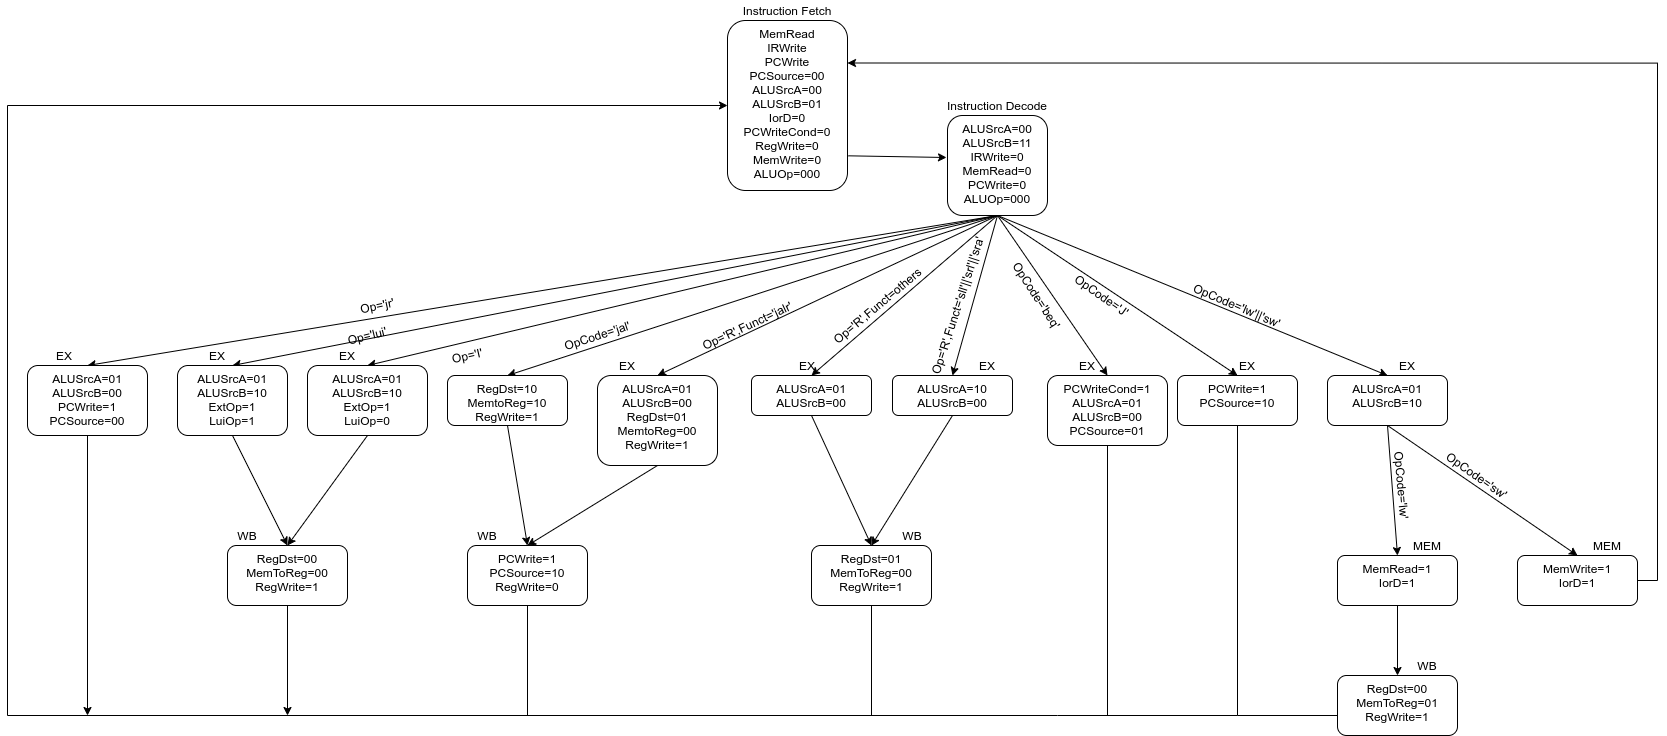
\includegraphics[width = 18cm]{images/fsm.png}
\end{center}


\section{ALU功能拓展}
\subsection{setsub类型和机器码字段内容}
setsub rd rs rt : \{6'h0,rs[4:0],rt[4:0],rd[4:0],5'h0,6'h28\}
\subsection{ALU verilog代码修改}
见代码附件。
\subsection{仿真结果}

\section{汇编程序分析-1}
\subsection{计算寄存器值}
\subsection{仿真结果}

\section{汇编程序分析-2}
\subsection{程序功能以及代码注释}
\subsection{将这段汇编翻译成机器码并写出}
\subsection{\$a0,\$v0值}
\subsection{观察、描述并解释 PC、\$a0、\$v0、\$sp、\$ra 如何变化}

\section{异常处理}

%\begin{lstlisting}[language=Matlab]
%\end{lstlisting}

\end{document}